%model-explore.v1

The spatio-temporal SSM encodes information about the abstract state
of the subject, the spatial maps corresponding to the state, the
state transition probabilities, and the hemodynamic response. In
addition, the optimal state-sequence for a particular fMRI session
(not necessarily the same as the one against which the SSM
parameters were estimated) can also be computed.

The \verb"params" object returned by \verb"ssmEstimateFull" (or by
\verb"ssmEstimate" encapsulates all the parameters of the SSM, which
can be explored by MATLAB code fragments. Addition, some helper
functions have also been provided, listed below.


\section{Computing Optimal State-Sequence}

This function estimates the optimal state-sequence by a specific
model for a given fMRI session.

Function Syntax:
\begin{verbatim}
    [st_seq_opt, log_likelihood ]
        = ssmGetStateSeq(params, fs_coords_session);
\end{verbatim}
Arguments:
\begin{itemize}
  \item \verb"params" - A structure of the SSM parameters as
  defined earlier.
  \item \verb"fs_coords" - The feature-space embedding of the fMRI session
\end{itemize}`
Returns:
\begin{itemize}
    \item \verb"st_seq_opt" - An array
    \item \verb"log_likelihood" - The log likelihood of the optimal
    state sequence
\end{itemize}


\section{State Marginal Distribution}
It is possible to compute the marginal probability distribution of
each state conditioned on a specific stimulus $\Pr[\x_t = k | \s_t]$
as follows

Function Syntax:
\begin{verbatim}
    [log_marginal ]
        = ssmStateMarginal(params, cond);
\end{verbatim}
Arguments:
\begin{itemize}
  \item \verb"params" - A structure of the SSM parameters as
  defined earlier.
  \item \verb"cond" - A structure giving the value of each stimulus
  (experimental conditions) for which the
  marginal is desired. Stimuli omitted from this structure are
  marginalized out. For example, let the names of the conditions
  as given in the \verb".mat" file created during
  the \verb"Specify 1-st Level" batch job of SPM,
  be \verb"stimulus_1" ... \verb"stimulus_n". If the distribution of
  state probabilities for \verb"stimulus_1"=5, \verb"stimulus_3"=2 are
  required, regardless of the other stimuli, then \verb"cond" will
  be
\begin{verbatim}
    cond.stimulus_1 = 5;
    cond.stimulus_3 = 2;
\end{verbatim}

\end{itemize}`
Returns:
\begin{itemize}
    \item \verb"log_marginal" - An array giving the log marginal probabilities for
    each state, under the specified experimental conditions.
\end{itemize}

This function can be used to generate plots giving the distribution
of each state during different experimental conditions, as shown in
\Fig{fig:state-trans}
\begin{figure}
     \centering
    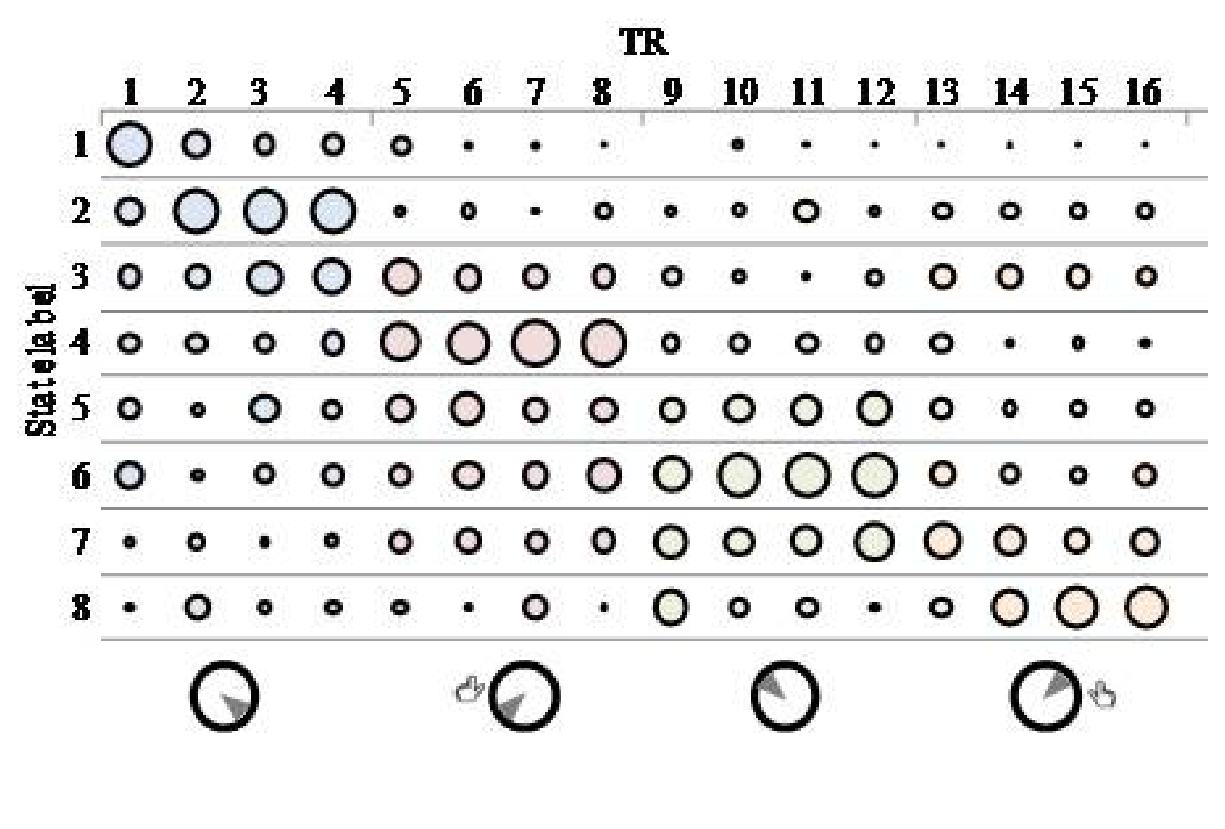
\includegraphics[width=\linewidth]{state-transition}
     \caption[Brain--State Probabilities]
     {\textbf{Brain--state probabilities for one subject.}
     The size of the
     circles corresponds to the marginal probabilities
     of the states during the display of the wedge in lower right,
     lower left, upper left and upper right quadrants for 4TRs each.
     States have been relabeled for expository purposes and
     transition probabilities have been omitted for visual clarity.}
    \label{fig:state-trans}
    \vspace{-.3cm}
\end{figure}


\section{Obtaining the State Transition Distribution}
Similar to the method above, it is possible to compute the entire
state transition probability matrix, conditioned on a specific
stimulus $\Pr[\x_{t} = j| \x_{t-1} = i , \s_t]$ as follows

Function Syntax:
\begin{verbatim}
    [log_transition]= ssmStateTransition(params, cond);
\end{verbatim}
Arguments:
\begin{itemize}
  \item \verb"params" - A structure of the SSM parameters as
  defined earlier.
  \item \verb"cond" - A structure giving the value of each stimulus
  (experimental conditions) for which the
  marginal is desired, as describe above.
\end{itemize}
Returns:
\begin{itemize}
    \item \verb"log_transition" - An 2D array giving the
    log probabilities for a state transition from
    state $i$ (row index) to state $j$ (column index),
    under the specified experimental conditions.
\end{itemize}





\section{The Activation Maps}
The spatially distributed activation pattern for a specific value of
the experimental variables along with its $z$--score map is computed
using the next function.

Function Syntax:
\begin{verbatim}
    [act_map_vi, z_map_vi ]  = ssmActivationMap(params, cond,
                            basis_set_idx, basis_filename);
\end{verbatim}
Arguments: Arguments:
\begin{itemize}
     \item \verb"params" - A structure of the SSM parameters as
      defined earlier.
  \item \verb"cond" - A structure giving the value of each stimulus
  (experimental conditions) for which the
  marginal is desired, as describe above.
    \item \verb"basis_set_idx" -
   The indices of the basis vector of the feature-space that
   retained after dimensionality reduction (\cf \Sec{sec:basc})
  \item \verb"basis_filename" -
    The filename of the 4D zipped NII (\verb".nii.gz")
    containing the basis vectors computed for a particular re-sample of the
    session.
\end{itemize}
Returns:
\begin{itemize}
    \item \verb"act_map_vi" - An \verb"spm_vol" structure giving the
    desired   activation map. Filename format is\\
    \verb"act_map_<cond_name_1>=<value>...<cond_name_n>=<value>.nii"
    \item \verb"z_map_vi" - An \verb"spm_vol" structure giving the
    desired   $z$-score map. Filename format is\\
    \verb"z_map_<cond_name_1>=<value>...<cond_name_n>=<value>.nii"
\end{itemize}
These $z$-score maps can be then examined and visualized either
volumetrically, or on inflated cortical surfaces (using FreeSurfer,
for example) as shown in \Fig{fig:mq-maps}.


\begin{figure}
%\begin{figure}%[h]
\centering
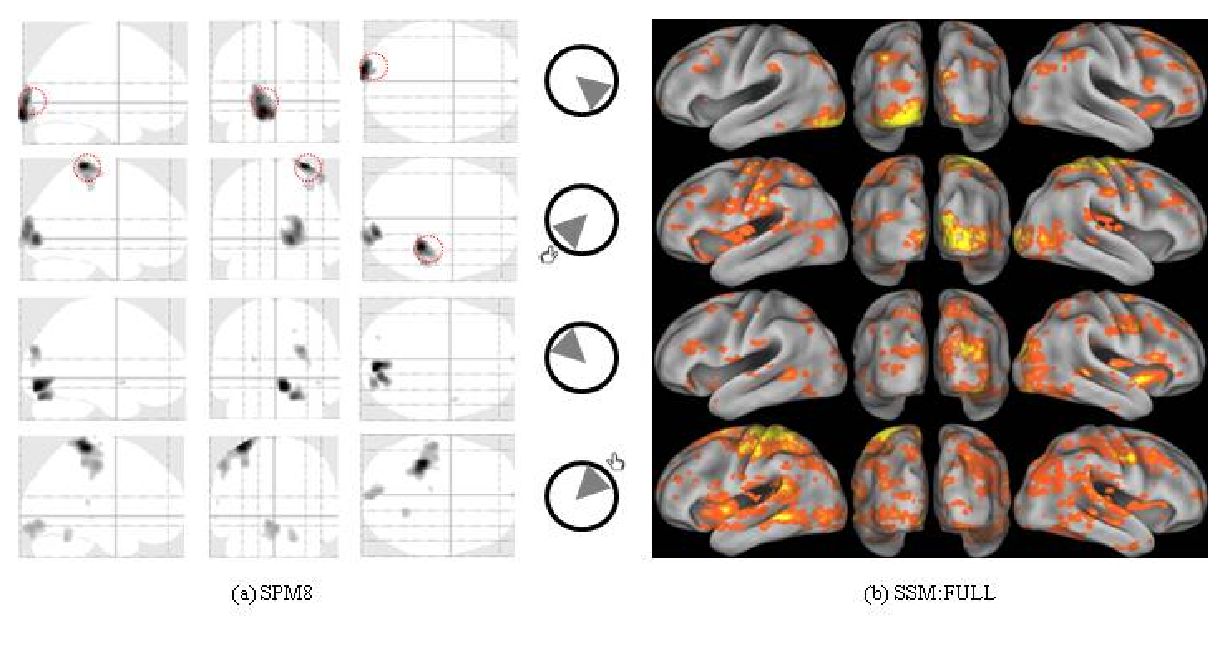
\includegraphics[width=\linewidth]{mq-maps}
\caption[Spatial Activation Maps ]{\textbf{Spatial Activation Maps
for the Visuo-Motor Task from SPM8 and the State--Space Multivariate
Analysis.} Fig.~(a): Maximum intensity projections of significantly
activated voxels ($p < 0.05$, FWE corrected) in a single subject for
the four orientations of the wedge and the hand motor actions,
computed using SPM8. The red circles indicate the ROIs for which the
estimated HR FIR filters are displayed in \Fig{fig:hrf-estimate}.
Fig.~(b): Spatial ($z$--score) maps showing the distribution of
activity for each orientation of the wedge computed from our
state--space model displayed on an inflated surface of the brain.
Displayed are the posterio-lateral and posterio-medial views of the
left and right hemispheres respectively. Values of $z \leq 1$ have
been masked out for visual clarity. }
 \label{fig:mq-maps}
\end{figure}



\section{The HRF Filters}
The SSM estimates an HRF filter at each feature-space coordinate.
These HRF estimates can be recombined and transformed back into the
original (physical) space to give the HRF estimated at a specific
location.

Function Syntax:
\begin{verbatim}
    [hrfs]  = ssmGetHRF(params, spatial_ijk,
                            basis_set_idx, basis_filename);
\end{verbatim}
Arguments: Arguments:
\begin{itemize}
     \item \verb"params" - A structure of the SSM parameters as
      defined earlier.
  \item \verb"spatial_ijk" - A $3\times n$ array giving the voxel
  coordinates (in $i-j-k$) at which the HRF estimates are desired.
    \item \verb"basis_set_idx" -
   The indices of the basis vector of the feature-space that
   retained after dimensionality reduction (\cf \Sec{sec:basc})
  \item \verb"basis_filename" -
    The filename of the 4D zipped NII (\verb".nii.gz")
    containing the basis vectors computed for a particular re-sample of the
    session.
\end{itemize}
Returns:
\begin{itemize}
    \item \verb"hrf" - An $n$ item array of the HRF filter
    coefficients for the desired spatial locations.
\end{itemize}

The HRFs can then be visualized as in \Fig{fig:hrf-estimate}


\begin{figure}[h!]
     \centering
 \mbox{
   \subfigure[Motor Cortex ROI]{
   \includegraphics[width=0.5\linewidth]{hrf_motor}
   }
    \subfigure[Visual Cortex ROI]{
    \includegraphics[width=0.5\linewidth]{hrf_visual}
    }
}
    \caption[Estimated Hemodynamic Response]
    {\footnotesize \textbf{Estimated hemodynamic FIR filter $\h$.}
    The estimated FIR filter coefficients for each of the four
    subjects averaged in two ROIs selected in the motor and visual cortices.
    \label{fig:hrf-estimate}
    }
\end{figure}
